%%%%%%%%%%%%%%%%%%%%%%%%%%%%%%%%%%%%%%%%%%%%%%%%%%%%%%
\chapter{Experimental design}
\label{experimental_design}
\graphicspath{{chapter_04/figures}{chapter_04/tables}}
%%%%%%%%%%%%%%%%%%%%%%%%%%%%%%%%%%%%%%%%%%%%%%%%%%%%%%


\section{Development of a flash-flood-focused verification framework}

This study faces two main challenges. The first challenge consists in the definition of the verifying thresholds that will be used to assess the performance of the rainfall-based and multi-parameter-based, data-driven predictions of areas at risk of flash floods. The second challenge consists of the use of appropriate verification scores due to the intrinsic characteristic of the observational datasets as it is not possible to define univocally observational yes- and non-events. 

In this section, we define a \textit{flash-flood-focused verification framework to assess (short- and medium-range) predictions of areas at risk of flash floods}. This framework will be used throughout the thesis to assess the performance of the rainfall-based flash flood forecasting system and its multi-parameter counterpart provided here by both data-driven models, the short-range (computed with the short-range ERA5 and ERA5-ecPoint forecasts) and the medium-range (computed with the equivalent long-range forecasts up to day 5). The application of the flash-flood-focused verification framework to the identification of areas at risk of flash floods involving solely rainfall predictions is done in the recognition that a robust understanding of rainfall forecast performance in identifying areas at risk of flash floods is essential to benchmark the performance of more advanced prediction methods, e.g. data-driven approaches involving more parameters.

The objective verification framework uses flash flood impact observations as ground truth. As indicated in section \ref{storm_event_database}, this thesis will consider only the Storm Event Database over the CONUS. However, this method can be applied in other geographical regions where regional databases are available, such as over Europe (using the ESWD dataset) or a global domain (considering global datasets such as EM-DAT), while always acknowledging the biases that such impact databases might possess. 


\subsection{Observational fields}
\label{obs_field}
The definition of the observational dataset follows the methodology proposed by \citep{Tsonevsky_2018} for severe weather, and \citep{Pillosu_2024} for flash floods in Ecuador. Each flash flood report was aggregated over the accumulation period for which the flash flood outlooks are provided. This thesis provides predictions of areas at risk of flash floods over 24-hourly accumulation periods starting at 00 UTC. Hence, this step's outcome consists of the list of \textit{point} flash flood reports happening between the 1st of January at 00 UTC and the 2nd of January at 00 UTC, between the 2nd of January at 00 UTC and the 3rd of January at 00 UTC, etc. 

Each point report in a specific accumulation period must then be located on the ERA5 grid-box where the event happened. In the Storm Event Database, the location of each flash flood event is provided by two latitude coordinates ("BEGIN\_LAT" and "END\_LAT") and two longitude coordinates ("BEGIN\_LON" and "END\_LON"). If BEGIN\_LAT = END\_LAT and BEGIN\_LON = END\_LON, the flash flood event is identified by a single point, and only the closest grid-box to that point is assigned the flash flood event using the "nearest grid-box" method. If BEGIN\_LAT \ne END\_LAT and BEGIN\_LON \ne END\_LON, a polygon is provided in all grid-boxes within that polygon get assigned the flash flood event. It is worth noting, that even when a polygon is provided, only one grid-box might contain the flash flood event is the radius of the event was not bigger than the ERA5's grid-boxes resolution, i.e., 31 km. This procedure creates \textit{gridded} fields of flash flood reports, where the values assigned to the grid-boxes indicate the number of flash flood reports occurred within the grid-boxes, e.g. a grid-box with 0 does not contain any flash flood reports for the considered accumulation period, while a grid-box with a value of 5 indicates that there are 5 flash flood reports within that grid-box, for the considered accumulation period.

Because of the large size of the ERA5 grid-boxes (i.e., 31 km) and the large accumulation periods for the flash flood outlooks (i.e. 24 hours), any additional expansion in the area or reporting times of individual reports is probably unnecessary to account for uncertainties in the location and reporting times as done in other studies \citep{Cavaiola_2024}. It is possible to envision remote scenarios in which a report is close enough to the edge of the ERA5 grid-box or the outlook accumulation period that a location or reporting time error in the database could cause the mislocation of such flash flood event, but this scenario has been established to be for ~0.1\% of the total number of the reports considered in this thesis, so no further methodologies will be considered here to account for uncertainties in the location or reporting time in the Storm Event Database. 

Figure \ref{fig:sed_reports} shows an example of the post-processed flash flood reports from the Storm Event Database.

\begin{figure}[htbp]
\centering
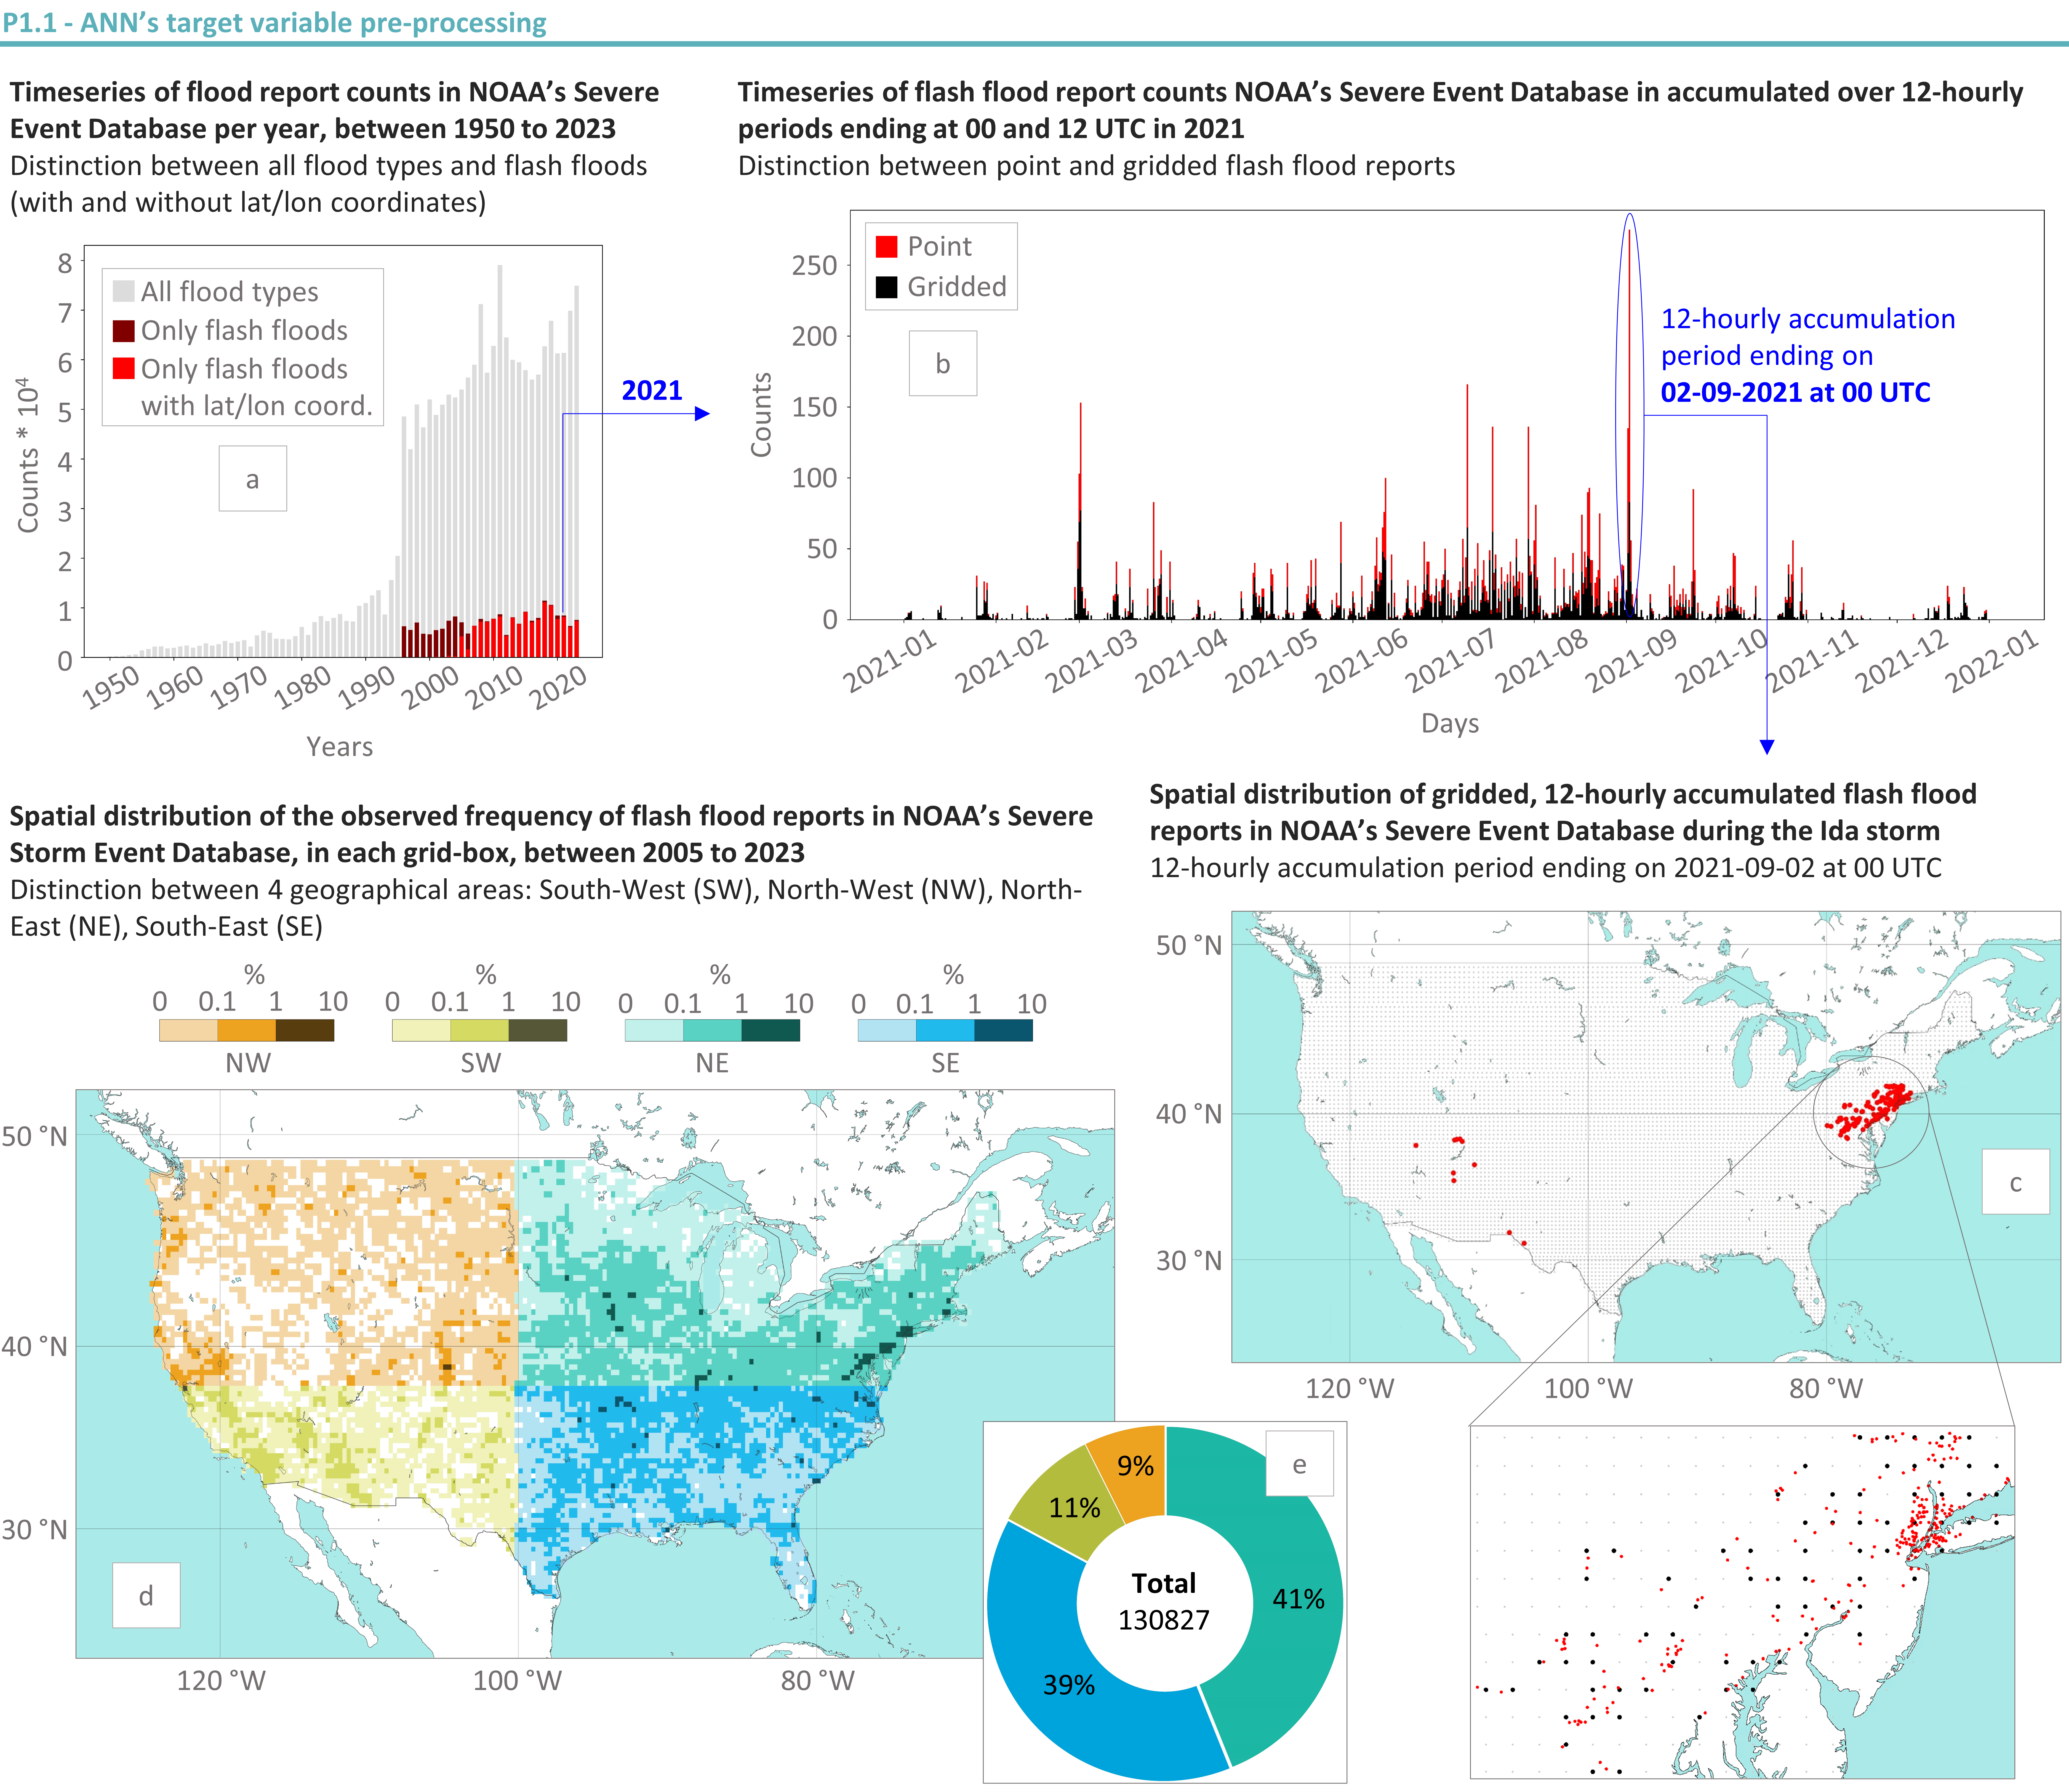
\includegraphics[scale=0.65]{sed_reports.png}
\caption{\textbf{Example of post-processed reports from the Storm Event Database.} Panel (a) shows the timeseries of the counts of all flood types recorded in the database from January 1950 to December 2023 (in grey), the counts of all flash floods recorded (in dark red), and the counts of all flash floods records including lat/lon coordinates (in red). Panel (b) shows the timeseries of point (in red) and gridded (in black) flash flood reports in 2021, accumulated over 12-hourly accumulation periods ending at 00 and 12 UTC. Panel (c) shows the spatial distribution of point flash flood reports (in red) during the 12-hourly accumulation period ending on 2021-09-02 at 00 UTC (i.e. for storm Ida). The zoomed in area shows an example of the number of point flash flood reports (in red) assigned to the nearest grid-box. Those grid-boxes containing at least one point flash flood reports is coloured in black. Panel (d) shows the spatial distribution of the observed frequency of flash flood events in each grid-box between 2005 and 2023. A distinction between four main areas is applied: the probabilities in the north-west, north-east, south-east and south-west are indicated, respectively, in orange, turquoise, cyan, and green. The probabilities are discretised in equal to 0\% (in white for all the regions), between 0-0.1\%, 0.1-1\%, and 1-10\% (in different tones of the colour for the corresponding region). Panel’s (d) insert shows a piechart representing the proportion of gridded flash flood reports in each considered region.}
\label{fig:sed_reports}
\end{figure}


\subsection{Forecast fields}

Given a forecast value at a grid-box, a flash flood event is considered as a yes-event if the forecast exceeds a specific event threshold (whose definition is explained in section \ref{verifying_rainfall_threshold}). The forecast fields are then created by assigning the value 1 to all those grid-boxes where the forecasts exceed the considered threshold; otherwise, the value 0 is assigned. 

\subsection{Definition of the verifying thresholds}
\label{verifying_rainfall_threshold}
For the rainfall-based predictions of areas at risk of flash flood, a rainfall-based threshold must be used. For the verification of rainfall-based predictions of areas at risk of flash floods, flash-flood-triggering rainfall totals might be known for the region of interest, so that they can be used as thresholds to define the flash flood events to verify. In this thesis, such rainfall thresholds are not know for the CONUS, and therefore, must be computed from data. If point rainfall observations are available (e.g., rain gauges or radars), one can create the distribution of the observed flash-flood-triggering rainfall totals, and the verifying rainfall thresholds (VRT) values would then correspond to the specific percentiles of the distribution. The higher the percentile, the higher the magnitude of the VRT, and the higher the severity level of flash flood events considered in the objective verification analysis. This approach requires high-density rainfall observations, in both space and time, to capture the localised extreme rainfall totals that trigger flash floods \citep{Haiden_2016, RamosFilho_2021}. In the absence of a suitable observational network, the VRT values can be defined only from gridded rainfall products such as reanalysis e.g., ERA5 \citep{Hersbach_2020}, reforecasts \citep{Hamill_2006b}, or blended rainfall observations provided on a grid such as MSWEP \citep{Beck_2019} or GPCP \citep{Adler_2018}. These datasets, however, tend to underestimate rainfall extremes because of their coarse spatial resolution \citep{Tapiador_2019}. In the absence of more suitable gridded datasets, \citet{Pillosu_2024} proposed a methodology to compute regional point rainfall climatologies using 1 year of short-range (day 1) ecPoint rainfall forecasts. This approach, however, has the disadvantage to use only 1 year of forecasts, which means that the resulting climatologies will inevitably be affected by the climatology of that specific year instead of the general climatology of the region that they are supposed to represent. Moreover, as this climatology requires flash flood observations to be defined, and such observations tend to have an even lower resolution than rainfall forecasts, there is the need to create climatologies for large domains, rather than on a grid-box scale. For example, \citet{Pillosu_2024} created only two verifying rainfall thresholds for Ecuador, one for the coastal and one for the Andean region. While this disaggregation is better than having one single value for an entire country, regional thresholds might not be able to capture flash-flood-triggering rainfall thresholds over different micro-climates. This would not allow an appropriate disaggregation of the performance of the flash flood forecasts in different regions, under different (hydro-meteorological) conditions. Hence, in this thesis, we propose the definition of the rainfall VRTS from a climatology built with ERA5-ecPoint rainfall estimates, as they have been shown to represent point-rainfall climatologies around the world reliably \citep{Pillosu_2025a} and they would allow us to develop a grid-box scale rainfall climatology to be used as thresholds for the rainfall-based predictions of areas at risk of flash floods. Hence, an ERA5-ecPoint rainfall climatology has been computed over the WMO recommended 30-year period 1991-2020 \citep{WMO_2017}. Table \ref{} shows the percentiles and corresponding values as x-year return periods that have been considered as flash-flood-triggering rainfall events during the verification.


\subsection{Objective verification}

The objective verification carried out in this thesis is based of verification scores computed through a probabilistic contingency table. We follow \citet{Pillosu_2024} methodology for the population of the contingency tables. Stationary observations (i.e. provided by instruments installed at a specific location, such as rain gauges, provide timeseries of yes- and non-events recorded at the location where the instrument was installed. THus, all four elements in the contingency table can be quantified. Non-stationary observations record only yes-events at the location where the event occurred. As a result, it is impossible to answer the question "if there are no reports in an area, is it because an event happened but nobody reported it, or because there was no event to report?". Some studies facing the same problem because they use non-stationary observations such as impact reports, verify only yes-events with the caveat that only quadrant I (i.e. hits) and III (i.e. misses) of the contingency table can be populated \citep{Robbins_2018}. Instead, this study followed the method proposed by \citet{Tsonevsky_2018}, which allows to populate all quadrants of the contingency table. This method assumes that a non-reports corresponds to a non-event. 

Hence, the contingency tables are built by examining overlapping grid boxes in correspondent observational and forecast fields. When both grid-boxes are assigned a value of 1 or 0, they count as a hit or a correct negative, respectively. When a grid-box in the observational field is assigned a value of 1, and the corresponding grid-box in the forecast field is assigned a value of 0, it counts as a miss. It counts as a false alarm if the opposite occurs. 


\subsection{Properties of probabilistic forecasts}

Reliability and discrimination ability are desirable properties of ensemble forecasts, and both are defined against a verifying threshold \citep{Jolliffe_2012, Wilks_2020}. Reliability measures whether the chosen verifying threshold is predicted with probabilities that mirror the frequency with which the considered event is observed. Discrimination measures the forecasts' ability to distinguish situations that lead to events exceeding the verifying threshold from those that do not, appraising the existence of a signal in forecasts when an event materialises. In this thesis, we consider two types of scores to analyse reliability and discrimination ability: summary and breakdown scores. Summary scores show the overall reliability and discrimination ability of the forecasts, while the breakdown scores provide detailed insights into how reliability and discrimination ability relate to the full distribution of probabilities. 


\subsubsection{Reliability}

To assess the overall reliability of the forecasts, we will consider the frequency bias (FB) to evaluate the overall reliability of the predictions of areas at risk of flash floods. The frequency bias was determined by dividing the total number of yes-events in the forecasts by the total number of yes-events in the observations. FB values range from 0 to $+\infty$. FB = 1 indicates perfect calibration, while scores greater or smaller than 1 indicate, respectively, over- and under-prediction of the observed yes-events. It is worth noting that FB measure the overall ratio of forecasts events to observed events and is not a measure of forecast sill. As such, it can provide a score of 1 when there are compensating error. Moreover, FB might show large overestimations if the observed event is heavily underreported. This is our case as explained in section \ref{fig:sed_reports}.

To break down the reliability of the forecasts over the full distribution of probabilities, reliability diagrams are used. They plot the relative forecasts probability of an event against its corresponding relative observational frequency, indicating how reliable the forecast probabilities are at different classes. For perfect forecasts, when the forecasts show x\% probability of occurrence, observations should meet the criteria x\% of the time, so that the reliability curve lies on the diagonal. If the reliability diagram is above the diagonal for a specific forecast probability, those forecasts are under-predicting the likelihood of observing a yes-event. If it lies below the diagonal, the is over-prediction. When analysing reliability diagrams, it is also important to know the frequency distribution of forecasts issued with specific probabilities. For example, the small probability thresholds (within the red box in the figure example) are the most important when considering high verifying thresholds because the sample of forecasts exceeding the verifying threshold with high probabilities is rather small. For this reason, reliability diagrams should be accompanied by sharpness diagrams, which plot the absolute frequency of forecasts of different probabilities. 


\subsubsection{Discrimination ability}

\begin{table}[htbp]
\centering
\captionof{table}{\textbf{Example of a 2x2 contingency table}. The table defines the four quadrants constituting a 2x2 contingency table.}
\includegraphics[width=\textwidth]{contingency_table.png}
\label{table:contingency_table}
\end{table}

Relative Operating Characteristic (ROC) curves are built from 2x2 contingency tables (Table \ref{contingency_table}), quantifying hits (H) misses (M), false alarms (FA), and correct negatives (CN). Hit rates (HR) and false alarm rates (FAR) are computed, respectively, from equations \ref{eq:hr} and \ref{eq:far}:

\begin{equation}
\mathrm{HR} = \frac{\mathrm{H}}{\mathrm{H} + \mathrm{M}}\quad[\text{values between }0\text{ and }1]
\label{eq:hr}
\end{equation}

\begin{equation}
\mathrm{FAR} = \frac{\mathrm{FA}}{\mathrm{FA} + \mathrm{CN}}\quad[\text{values between }0\text{ and }1]
\label{eq:far}
\end{equation}

HRs are mapped (Y-axis) against FARs (X-axis) in a unit square. The form of the ROC curve shows how HRs vary with FARs as one systematically lowers the thresholds probability at which it is assumed that an event has technically been forecast to happen (i.e. 100\% of probability the bottom left corner to 0\% probability at the top right corner). The values of the geometrical area under the ROC curve (AROC) provide a summary measure of the discrimination ability across all probability thresholds. The plot of AROC values for different lead times allows us to compare the discrimination ability between the rainfall-based predictions of areas at risk of flash floods, and the multi-parameter-based, data-driven predictions, (both at short- and medium-range lead times). Perfect discrimination is obtained when only HRs grow and FARs remain zero. It is represented by a ROC curve that rises along the Y-axis from the bottom left corner of the unit square to the top-left corner and moves straight to the top-right corner. In this case, the AROC is equal to 1. If HRs and FARs grow at the same rate, the forecasts have no discrimination ability (as a climatological forecast). In this case, the ROC curve lies along the diagonal and AROC equals 0.5. 

How ROC curves and AROCs are computed can impact the interpretation of forecasts discrimination ability. For rainfall-based predictions, the ROC curves will be built for incremental decision thresholds that are materially assessable from the real ensemble configuration. In this way, we can estimate the "real" forecast discrimination ability \citep{wilks_statistical_2020}. Probability thresholds are determined by considering the full discretisation ability in the ensemble (e.g., 99 members in the case of ERA5-ecPoint). This ensures that the ROC curves are as complete as possible \citep{Bouallegue_2022}. The number of thresholds corresponds, therefore, to the number of members exceeding the verifying rainfall threshold so that for an enmble of size M, maximum discretisation is achieved by M+1 probability thresholds (i.e., 0, 1/M, 2/M, ...., M/M=1). For the data-driven forecasts, where the forecast probability is provided by the model with continuous numbers between 0 and 1, the decision (probability) thresholds are defined by the user. In this thesis, a discretisation of 0.01 (equivalent to 1\%) and 0.001 (equivalent to 0.1\%) will be considered given the low frequency observed of flash flood events in the observational database. The ROC curve is then built by straight segments joining successive points. It is then completed by joining that last meaningful point with a straight line in the top-rigth corner of the unit square. For rare events, the points of a ROC curve cluster in the graph's bottom left corner and completing the ROC with a straight line might give the impression that part of the curve is missing \citep{Casati_2008}. How much the curve appears incomplete depends on the ensemble size and the base rate of the event. The area under the ROC curve (AROC) will be computed using a trapezoidal approximation by adding the areas of single trapeziums formed by the straight lines between consecutive points in the ROC curve \citep{Bouallegue_2022}. 

From what written before, the ROC curves represent the breakdown measure of discrimination ability as it will be possible to examine the values of HRs and FARs at different decision (probability) thresholds. AROC will represent instead the overall measure of discrimination ability.


\section{Development of the multi-parameter data-driven forecasts of areas at risk of flash flood}

Traditional physically-based models, which rely on physical equations and mathematical models, are the backbone of many scientific disciplines for decades. These algorithms are based on well-established principles and laws of physics, enabling a systematic and predictable approach to problem-solving. On the other hand, AI-based strategies emerge as a powerful tool for handling vast amounts of data and extracting patterns and relationships that might be challenging to identify through traditional algorithms.

Over the years, semi-empirical, index-based models have provided predictions of areas at risk of flash floods up to continental scales \citep{Ma_2021} and medium-range lead times \citep{Alfieri_2015a, Raynaud_2015}. However, their extension to a global domain remains difficult because to set all free parameters over a region of interest or global domain, a large amount of flash flood observations (either form discharge gauges or impact reports) are needed and, to this day, this is a requirement still difficult to satisfy being flash floods rare events, happening typically in ungauged catchments, and being largely underreported in impact databases. 

Alternative strategies to deal with the issue of forecasting exploit data-driven-based predictions, defined as predictions made solely in terms of the knowledge of field data. Recently, data-driven methods have shown potential in accelerating weather forecasting by orders of magnitude, even if the accuracy of the forecasts is not always higher than that of NWP models \citep{Bauer_2021}. To date, there are a series of data-driven models that learn meteorological \citep{Lang_2024} and hydrological \citep{Nearing_2024} dynamics from ERA5 global reanalysis. However, ERA5 does present limitations in reconstructing sub-grid features due to the coarse spatial resolution, inherent biases in the model, and sub-grid processes that are only parametrised in the NWP model \citep{Pillosu_2025a}. Hence, the same skills shown in previous literature should not be taken for granted when the focus is on the representation of phenomena that occur at sub-grid scale or for extreme events (e.g. rainfall events exceeding, for example, the 20-year return period or larger thresholds).

Data-driven approaches have been used widely to forecast flash flood events, but primarily up to 24-hours ahead and solely at catchment \citep{Zhao_2025, Saleh_2024, Oddo_2024}, regional \citep{Deijns_2024}, and national level \citep{Villacca_2025, Zhao_2022}. While achieving very good verification scores (for example AROC scores > 0.8), the use of such data-intensive, data-driven algorithms, such as deep neural networks is not possible for global applications. While recent wisdom advocates for using hydro-meteorological data for a number of catchments available around the world to train a single model that later can be used to provide seamless flood forecasts around the world \citep{Kratzert_2024}, the application of similar strategies is restricted for flash flood applications due to the rather small number of data available for flashy catchments around the world e.g., 1\% of catchments in the CARAVAN database have an area below <100 km2 \citep{Kratzert_2023}. Even including more recent extensions of the CARAVAN database, such the percentage of data for flashy catchments does not exceed 5\% of the full database \citep{Färber_2024}.

Less data-intensive machine learning algorithms, such as decision-tree-based algorithms, such as random forest and boosting, and shallow feed-forward neural networks, could help to model the non-linear relationships between the hydro-meteorological parameters and create predictions of areas at risk of flash floods even when using low-density impact flash flood impact databases. The aim is to train the data-driven model with the higher-resolution Storm Event Database and apply it globally to provide predictions over a continuous global domain, for short-range forecasts (up to day 1) using ERA5 short-range forecasts (aka reanalysis) and for medium-range forecasts (up to day 5) using ERA5 long-range forecasts.

\subsection{The challenge of imbalanced observational datasets}

\subsubsection{Ensemble techniques}
The resulting observational dataset, built as described in section \ref{obs_field} is strongly imbalanced, with only 0.2\% of yes-events over the whole training+testing period (from 2001 to 2024). Using a similar dataset for the learning stage of our data-driven model is challenging, as the model might learn that non-events should always be predicted, as the model sees too few yes-events compared to the non-events, so that the model gives up on predicting the yes-events \citep{Haixiang_2017}. To overcome this problem, different techniques at data-level or algorithm-level are available \citep{Altalhan_2025}. 

Data-level balancing techniques focus on aligning class distributions by adjusting the size of training datasets through resampling, which aims to equalise the class distribution through "undersampling" or "oversampling" approaches. Standard undersampling techniques include Random Undersampling, Tomek, and cluster centroids, while prominent oversampling techniques include SMOTE and derivatives like Borderline-SMOTE and ADASYN \citep{DeVargas_2023}. However, these approaches introduce two main challenges: oversampling may lead to overfitting, reducing generalisation on the test set, whereas undersampling may result in a significant loss of knowledge from the majority class (i.e. non-events). Generative Adversarial Networks (GANs) are also used to improve the classification accuracy of imbalanced datasets. Oversampling and GAN techniques generate synthetic samples and the verification of how their distribution if to that of the original dataset is very difficult due to the lack of real observational data. Hence, we might be training models with data that does not respect the frequency distribution of yes-(flash flood)events.

Algorithm-level techniques enhance learning in the minority class by immediately altering the training process of the classifier or modifying algorithms to address challenges associated with imbalanced datasets \citep{Altalhan_2025}. Algorithm-specific adjustments like adapting class-balanced loss functions for gradient Boosting Decision Trees have shown high effectiveness in addressing class imbalance \citep{Luo_2025}. Ensemble methods entail merging multiple base classifiers or models to forge a more robust learner to address the imbalance problem, such as random forest, gradient boosting, bagging, and stacked learning. These approaches leveraged various algorithms or versions of the same model (e.g. for extreme gradient boosting, different version of the same algorithm can be, for example, XGBoost and LightGBM) to bloster predictive performance on imbalance datasets. 

In this thesis we do not apply data-level balancing techniques because we do not want to introduce uncertainties in the estimation of the forecasts by pre-processing the training dataset, either creating synthetic data over oversampling, or eliminating possibly information-riched non-event data-points. To not introduce uncertainty in the predictions, we will not consider algorithm-specific adjustments either. To consider these techniques robustly, a thorough assessment of each technique would be needed, using predictions from models trained on the original "real" observations as a benchmark to assess any gain or loss of predictive performance in the models trained with modified training datasets or modified algorithms. This work is out of the scope of this thesis. For future work in this field, the results produced in this thesis might serve as benchmark for those predictions. Hence, in this study, we will consider ensemble techniques to address the problem of having an extremely imbalnce dataset, and the models mentioned in Table \ref{} will be used. 


\subsubsection{Stratified k-fold cross validation}

Instead of assessing the robustness of the learning process by dividing the observational dataset into training, validation, and test sets, training only once over the training dataset and evaluating the model only once over the validation and test dataset, we opted for a validation strategy that allows for controlling the robustness of the inference phase. A well-established approach for this scope is the " stratified k-fold cross-validation", where possible biases caused by a fortunate/ unfortunate choice of the test dataset are mitigated by selecting different training, validation, and test datasets at each iteration. 
